%%%%%%%%%%%%%%%%%%%%%%%%%%%%%%%%%%%%%%%%%
% Classic Lined Title Page 
% LaTeX Template
% Version 2.0 (22/7/17)
%
% This template was downloaded from:
% http://www.LaTeXTemplates.com
%
% Original author:
% Peter Wilson (herries.press@earthlink.net) with modifications by:
% Vel (vel@latextemplates.com)
%
% License:
% CC BY-NC-SA 3.0 (http://creativecommons.org/licenses/by-nc-sa/3.0/)
% 
% This template can be used in one of two ways:
%
% 1) Content can be added at the end of this file just before the \end{document}
% to use this title page as the starting point for your document.
%
% 2) Alternatively, if you already have a document which you wish to add this
% title page to, copy everything between the \begin{document} and
% \end{document} and paste it where you would like the title page in your
% document. You will then need to insert the packages and document 
% configurations into your document carefully making sure you are not loading
% the same package twice and that there are no clashes.
%
%%%%%%%%%%%%%%%%%%%%%%%%%%%%%%%%%%%%%%%%%

%----------------------------------------------------------------------------------------
%	PACKAGES AND OTHER DOCUMENT CONFIGURATIONS
%----------------------------------------------------------------------------------------

\documentclass[a4paper, 12pt, oneside]{book} % A4 paper size, default 11pt font size and oneside for equal margins

\usepackage[svgnames]{xcolor} % Required for colour specification

\newcommand{\plogo}{\fbox{$\mathcal{PL}$}} % Generic dummy publisher logo

\usepackage[utf8]{inputenc} % Required for inputting international characters
\usepackage[T1]{fontenc} % Output font encoding for international characters
\usepackage{fouriernc} % Use the New Century Schoolbook font
\usepackage{enumerate}

%%%%%% Basic packages begin %%%%%%
\usepackage[
textwidth  = 160mm, 
textheight = 230mm, 
top        = 25mm, 
bottom     = 30mm
]{geometry}
\usepackage[normalem]{ulem}
\usepackage[utf8]{inputenc}
\usepackage[T1]{fontenc}
\PassOptionsToPackage{defaults=hu-min}{magyar.ldf}
\usepackage[magyar]{babel}
\usepackage{graphicx,wrapfig,lipsum}	
%%%%%%% Basic packages end %%%%%%%

%%%%%% Packages required for this document begin %%%%%%
\usepackage{
	amsmath,   % Math mode
	amsthm,    % "note" environment
	amsfonts,  % "\mathbb{}" command
	paralist,  % "compactitem" and "compactenum" environment
	multirow,  % "\multirow{}{}" command
	float,     % "H" float specifier
	tikz,      % Basepackage for nearly all figures
	listings,  % Used for code snippets
	etaremune, % Reverse compactenum
	%	graphicx   % For including images
	enumitem   %for alphabetical enumeration
}
\usepackage[unicode]{hyperref} % Clickable links
%%%%%%% Packages required for this document end %%%%%%%

%%%%%% TikZ options start %%%%%%
\usetikzlibrary{
	positioning, % Contains positioning utilities, such as "below = of" 
	calc,        % Adding coordinates
	math         % Needed for global variables
}

\tikzstyle{NodeBase} = [
rectangle,
text centered,
draw = black
]

\definecolor{DefaultObjectColor}{gray}{0.9} % This is the default color of object in the TikZ pictures

\tikzstyle{arrow} = [
thick,
->,
>=stealth
]
%%%%%%% TikZ options end %%%%%%%

%%%%%% lstlistings envvironment options start %%%%%%

\lstdefinestyle{customc}{ % C/C++ code snippet style
	belowcaptionskip = 1\baselineskip,
	breaklines       = true,
	frame            = L, % Double line on the left
	language         = C++,
	showstringspaces = false,
	basicstyle       = \ttfamily,
	keywordstyle     = \bfseries\color{green!40!black},
	stringstyle      = \color{orange},
	emphstyle        = \color{blue}, % Defined below
	tabsize          = 4,
	columns          = fullflexible,
}
\renewcommand{\thesection}{\Roman{section}} 
\renewcommand\thesubsection{\arabic{subsection}}
\setcounter{section}{0}

\begin{document} 

%----------------------------------------------------------------------------------------
%	TITLE PAGE
%----------------------------------------------------------------------------------------

\begin{titlepage} % Suppresses headers and footers on the title page
	
	\centering % Centre everything on the title page
	
	%------------------------------------------------
	%	Top rules
	%------------------------------------------------
	
	\rule{\textwidth}{1pt} % Thick horizontal rule
	
	\vspace{2pt}\vspace{-\baselineskip} % Whitespace between rules
	
	\rule{\textwidth}{0.4pt} % Thin horizontal rule
	
	\vspace{1cm}
	%\vspace{0.1\textheight} % Whitespace between the top rules and title
	
	%------------------------------------------------
	%	Title
	%------------------------------------------------
	
	\textcolor{DarkBlue}{ % Red font color
		{\Huge \textsc{\textbf{Jaschik Álmos Művészeti Szakközépiskola}}}\\
		\vspace{1cm} % Title line 1
		{\Huge Festészet elmélet}\\[0.5\baselineskip] % Title line 1
		{\Large jegyzet}\\[0.5\baselineskip] % Title line 2
	}
	
	\vspace{0.025\textheight} % Whitespace between the title and short horizontal rule
	
	\rule{0.3\textwidth}{0.4pt} % Short horizontal rule under the title
	
	\vspace{0.1\textheight} % Whitespace between the thin horizontal rule and the author name
	
	%------------------------------------------------
	%	Author
	%------------------------------------------------
	
	{\Large \textsc{\textit{Készítette: Csonka Szilvia}}}\\ % Author name
	\vspace{1cm}
	{\Large \textsc{Balogh Ede Farkas órái alapján}} % Author name
	
	\vspace{1cm}
	%\vfill % Whitespace between the author name and publisher
	
	%------------------------------------------------
	%	Publisher
	%------------------------------------------------
	\begin{figure}[h!]
		\centering
		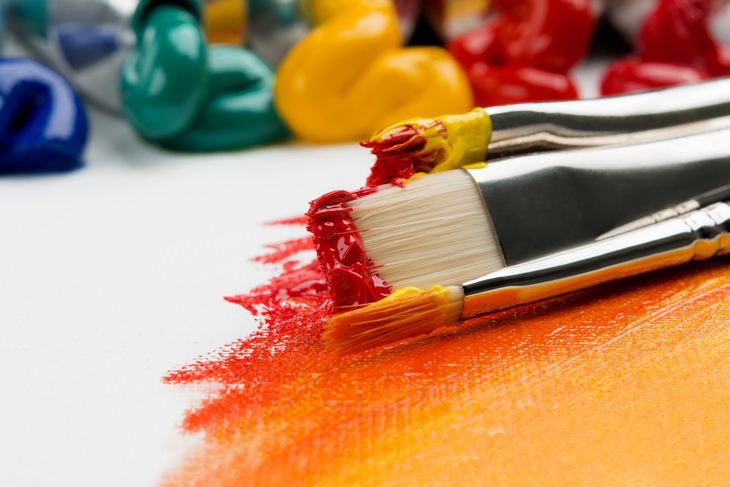
\includegraphics[width=0.9\linewidth]{cover}
	\end{figure}
	
	%{\large\textcolor{Blue}{\plogo}}\\[0.5\baselineskip] % Publisher logo
	
	%{\large\textsc{the publisher}} % Publisher
	
	%\vspace{0.1\textheight} % Whitespace under the publisher text
	
	%------------------------------------------------
	%	Bottom rules
	%------------------------------------------------
	
	\rule{\textwidth}{0.4pt} % Thin horizontal rule
	
	\vspace{2pt}\vspace{-\baselineskip} % Whitespace between rules
	
	\rule{\textwidth}{1pt} % Thick horizontal rule
	
\end{titlepage}

%----------------------------------------------------------------------------------------

\section{Az őskori barlangfestményekhez használt  anyagok, pigmentek, kötőanyagok, technikák}

	\subsection{A tétel teljes címe}
	
	Melyek azok az anyagok, pigmentek, kötőanyagok, amelyek az őskori barlangfestmények készítőinek rendelkezésére állhattak? Milyen alapvető lépésekből állhatott a kivitelezés módja a barlangfestmények elkészítésekor?
	
	\subsection{Bevezetés}
		A festészet kialakulása, tekintetbe véve a barlangfestmény leleteket, egészen az emberiség őskoráig nyúlik vissza. Az ősember a természetben található pigmenteket, használta a barlang rajzok színesebbé tételére, ill. esetleg kultikus célokra. A rendelkezésére álló színek mennyisége és tartománya igen korlátozott volt, elsősorban színes földfestékekről és faszénről beszélhetünk.
		
		Az első művészeti alkotások 30 000 évvel ezelőtti időből származnak. A leghíresebbek a
		barlangfestmények; ma mintegy 200 őskori falfestményt rejtő barlangot ismerünk. A
		leghíresebb barlangok a franciaországi \textbf{Lascaux-barlang}, illetve a spanyolországi \textbf{Altamira-barlang}.
		Magyarországon a \textbf{Szeleta-barlang}ban található barlangfestmény.
		A barlangrajzok alapvető jellemzője, hogy az állati alakokat – többnyire bölényeket,
		vadlovakat, szarvasokat - a legjellemzőbb nézetből, oldalirányból ábrázolták, és mozdulat
		közben. Nem az apró részleteket adják vissza, hanem a lényeget leegyszerűsített formában.
		Tudatos kompozíció és szerkesztés hiányzik. Színezéshez vörös, sárga, fekete színeket
		használtak; a porrá zúzott anyagokat vízzel, zsírral, vérrel elkeverve vitték fel a falra. 
	
	\subsection{Az őskor részei}
	
	\begin{enumerate}
		\item Neander-völgyi ember művészete: Kr. e. 150 ezer-től Kr. e. 15 ezer-ig.
		\item Paleolitikum: Kr. e. 15 ezer - Kr. e. 9-8 000-ig.
		\begin{compactitem}
			\item "paleo" = "ős", "lito" = "kő" $\rightarrow$ "őskőkor"
			\item \textit{Megjegyzés: főleg ez az időszak a jelentős számunkra.}
		\end{compactitem}
		\item Neolitikum: Kr. e. 9-8 ezer - Kr. e. 3000 (újkőkor)
	\end{enumerate}
	
	\subsection{Melyek azok az anyagok, pigmentek, kötőanyagok, amelyek az őskori barlangfestmények készítőinek rendelkezésére állhattak?}
	
		\subsubsection{Pigmentek}
		
		Főleg a természetben megtalálható, föld pigmenteket használtak, sokszor kötőanyag nélkül, por vagy rög formájában. Példák:
		\begin{compactitem}
			\item fehér agyag $\rightarrow$ fehér szín
			\item vasoxid és mangánoxid $\rightarrow$ okker, barna és vörös (hőfoktól függően)
			\item égetett csont és faszén $\rightarrow$ fekete
		\end{compactitem}
	
		\subsubsection{Kötőanyagok}
		
		Az őskori barlangfestményekhez használt kötőanyagok -- akárcsak a pigmentek -- a természetben megtalálható anyagok voltak.Például:
		\begin{compactitem}
			\item emberi vagy állati vér $\rightarrow$ érdekesség, hogy az emberi vér 10 000 év elteltével is megtart valamit a pigmentből
			\item viasz $\rightarrow$ az igazoltan legkorábbi viasszal készült kép egy teknősbékát ábrázol
			\item zsiradék (faggyú)
			\item tej (neolitikum)
		\end{compactitem}
		
		Sokszor kötőanyag nélkül is használták a pigmenteket. Valamilyen tálból, vagy kagylóhéjből fújták fel a porpigmentet a falra vagy pigmenttömb (pl. széndarab vagy agyagtömb) segítségével, azt krétaként használva vitték fel a színt.
		
		\subsubsection{Természetes freskósodás}
		
		A mészkő barlang falának felületén széndioxid hatására természetes folyamat következtében az évek során vékony mészkőréteg, mészkőpáncél keletkezik. 
		
		Az őskori barlangfestményeket, barlangrajzokat ez a folyamat konzerválta: a mészkőfalra felvitt pigment tetején kialakuló cseppkőréteg megkötötte a pigmentet és konzerválta a falfestményeket.
		
		
	\subsection{ Milyen alapvető lépésekből állhatott a kivitelezés módja a barlangfestmények elkészítésekor?}
		
		\subsubsection{Technikák}
		
		A barlangábrák főként vonalakból, színezett felületekből, éles kontúrokból tevődnek össze.
		
		\begin{itemize}
			\item \textbf{Vonalak felvitele}\\
			Kréta szerű pigmenttömbökkel, pl. magas vastartalmú vagy vasoxidot tartalmazó rög segítségével barna, fekete, vörös és okker színű vonalak vihetőek fel.
			
			\item \textbf{Színezett felületek kialakítása}\\
			Összetördelt porfesték kagylóhéjból, vagy egyéb edényből a falra fújása pl. nádszál segítségével.
			
			\item \textbf{Éles kontúrok kialakítása}\\
			Maszkolás segítségével. Például két deszka közötti résbe fújva a pigmentet megkapjuk azok lenyomatát.
			
			\item \textbf{Tubfolás}\\
			Pigmentebe mártott bőrdarabokkal a pigment nyomdaszerű felvitele a falra. Például ilyen módszerrel kézlenyomat felvitele a falra. (Szignatúraként, nyomhagyás céljából.)
		\end{itemize}
	
		\subsubsection{Jellemzői}
		
		\begin{compactitem}
			\item Valószínűsíthetően főleg egy ember készítette el őket. 
			\item A falfestményeknek felépítése van, nagy barlangrészek vannak kialakítva velük.
			\item Főleg sámánok késíztették.
			\item Egyes kisebb részeket talán tanoncok készíthettek.
			\item Rendszerezés, pl.: egymással párosodni képes állatok egy helyre kerültek.
			\item Monumentalitás: nagy felületen voltak.
		\end{compactitem}
		
		\subsubsection{Lascaux-barlang}
		
		A barlangot be kellett zárni a látogatók előtt, mivel a fokozott széndioxid mennyiség felgyorsította a természetes freskósodás folyamatát és kezdtek eltűnni a barlangrajzok a falakról a rájuk rakódott vastag cseppkőréteg miatt.
		\begin{figure}[h!]
			\centering
			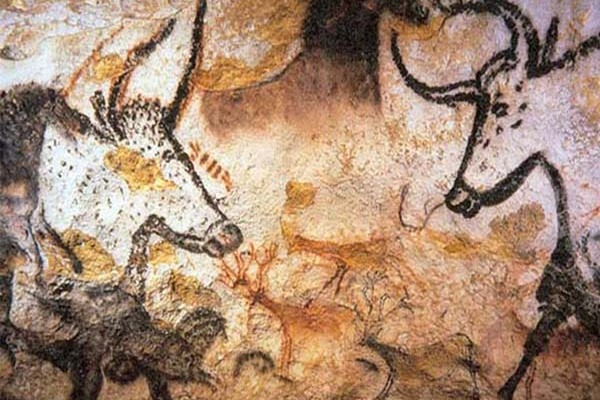
\includegraphics[width=0.7\linewidth]{lascaux-barlang}
			\caption{Lascaux barlang}
			\label{fig:lascaux-barlang}
		\end{figure}
		
\newpage 

\section{Meghatározó festészeti technikák az ókorban, az egyiptomi falkép}

	\subsection{A tétel teljes címe}
	
	Melyek a meghatározó festészeti technikák az ókorban? Fejtse ki, miként alakult egy egyiptomi falkép elkészítésének munkamenete, milyen alapozást, pigmenteket és kötőanyagokat használtak?
	
	\subsection{Anyaghasználat az ókorban}
	
	Az ókor több szempontból is áttörést jelentett a festészet szemszögéből nézve. Az ember már ismeri a kötőanyagok fogalmát a festészetben, így olyan festékeket hoz létre, melyek tartós filmréteget képeznek, akár 2000 év elteltével is jó állapotban fennmaradtak, pl. Fayum múmia portrék, Pompeji faliképek stb. 
	
	Kötőanyagnak elsősorban\textbf{ tojást, enyvet, viaszokat és néha növényi olajat} használtak.
	
	Továbbá képes bonyolultabb fizikai és kémiai folyamatokkal új színes pigmenteket létrehozni, pl. ólomfehér, mínium, egyiptomi kék stb.
	
	Az ókori ember már képes volt különböző, sokszor egészen bonyolult eljárásokkal létrehozni bizonyos színes pigmenteket, melyek addig nem álltak rendelkezésére. Pl. Ólomfehér, mínium, egyiptomi kék stb.
	
	\subsection{Festészeti technikák az ókorban}
	\subsubsection{Egyiptom}
	
	Egyiptom az ókori folyami kultúrák közé tartozó, gazdag és erős ország volt. A Nílus mentén
	elterülő Alsó- és Felső-Egyiptom i.e. 2900-ban egyesült Ménész fáraó uralma alatt. Az ókori
	Egyiptom történetét – ahogy a művészetét is korszakoljuk – három részre lehet osztani,
	megkülönböztetve az uralkodókat, uralkodóházakat: az Óbirodalom (i.e. 2650-2150; III-VI.
	dinasztia), a Középbirodalom (i.e. 2100-1750 körül, XI-XII. dinasztia), az Újbirodalom (i.e. 1550-
	1070, XVIII-XX. dinasztia) kora. Egyiptom hanyatlani kezdett, i.e. IV. században Nagy
	Sándor hódította meg.
	Egyiptom nagyságához hozzájárult, hogy korán kialakult egy egységes írásrendszer, amely
	elég fejlett volt nemcsak a mindennapi életben szükséges dolgok feljegyzéséhez, hanem a
	tudományos felfedezések és az irodalmi alkotások leírásához is. Az egyiptomiak hite szerint a
	halhatatlanságot az biztosította valaki számára, ha neve fennmaradt, ezért a legtöbben
	igyekeztek legalább a nevüket feljegyeztetni a sírkamrákban.
	Az egyiptomi írásrendszer megfejtése igen sokat segített az egyiptomi kultúra feltárásában, az
	egyiptológia, mint tudományág kialakulásában. A hieroglifák bonyolult képírás, melyben
	minden kis képnek külön jelentése van. A megfejtését a francia Jean-François Champollionnak köszönhetjük. 
	
	\subsubsection{Az egyiptomi festészet}
	
	Az élet mindennapi eseményeit örökítették meg, de általánosított, elvont formákkal. Az
	alakok mérete változott, mégpedig aszerint, hogy milyen rangja volt életében.
	A festmények a sziklasírokban, koporsókon fordultak elő. Jellemző rájuk, hogy az alakokat
	szigorú szabályok szerint festették meg: nincs egységes nézőpont, több nézőpontból (oldal-,
	elölnézet) ábrázolták ezeket. (legnagyobb felület törvénye). A síkszerű ábrázolás, szalagszerű
	kompozíció, az egymás feletti elrendezést tiszta élénk színekkel emelték ki még jobban. 
	
	
	\subsubsection{Ábrázolás az egyiptomi festészetben}
	
	Az egyiptomi művészetben az alakok, tárgyak síkban való ábrázolására a III. dinasztia elején szigorú szabályok alakultak ki, amelyek végig megmaradtak. A művészek meghatározott mintákből dolgoztak. Az alakok megszerkesztéséhez négyzethát alkalmaztak, ezáltal mind az alakok, mind a hireoglif jelek a rögzített arányrendszer szerint készültek. A művészeknek sok szabályt kellett megtartaniuk. Nem kívánták tőlük, hogy újat alkossanak, sőt, valószínűleg azt a művészt becsülték a legtöbbre, akinek munkái legjobban hasonlítottak a régi alkotásokhoz. Ebből a felfogásból adódott, hogy 3000 év alatt művészetük alig változott.
	
	A témákat megváltoztathatták, de az előadás módja, karaktere, lényegileg azonos maradt. Ennek alapján lehet ókori egyiptomi stílusról beszélni. Úgy képzelték, hogy a másvilágon a sírkamrákba helyezett szobrok dolgoznak az elhunyt helyett. A legtöbb alkotások sírokból kerültek elő: festmények a sírkamra falán, a halott szarkofágján, a halottakat a túlvilágon szolgáló szobrok és a neki odahelyezett edények, bútorok, a vele eltemetett ékszerek.
	
	Jellemzői: nincs árnyékolás, különböző nézőponti ábrázolás, állatok ábrázolása, térbeliség ábrázolása, stilizálás, díszítés, nem a látszat szerint festettek hanem a törvények alapján, templomok festése, egymás utáni szituációk ábrázolása.
	
	
	\subsubsection{Az egyiptomi festészet jellemzői}
	\begin{compactitem}
		\item Érvényesül a \textbf{legnagyobb felület törvénye}: az arc,  kar, a láb oldalnézetben van, a szem, a váll, a mellkas és törzs pedig elölnézetben, csípő 3/4 profilban.
		\item Kanonizált és jelképes (a fej mindig profilban van, a szem szemből, a törzs deréktól
		fölfelé elölnézetben, a mell oldalról, a test csípőtől lefelé szintén oldalról látszik stb.)
		\item A jeleneteket síkban kiterítik.
		\item Képregényszerű jelenetek.
		\item Az egymás mögöttiséget egymás fölöttiséggel helyettesítik.
		\item A mozgás mindig arra tart amerre mutatnak a képcsíkok.
		\item Nincs egyetlen nézőpont és térbeli mélység.
		\item A színek tiszták, élénkek. Használják a barnát, okkert, sárgát, kéket, zöldet, pirosat,
		feketét, fehéret.
		\item A képeknek van ritmusuk.
		\item Az alakok részben takarhatják egymást.
		\item Eszköz: földfesték, nádecset.
	\end{compactitem}

	\begin{figure}[H]
		\centering
		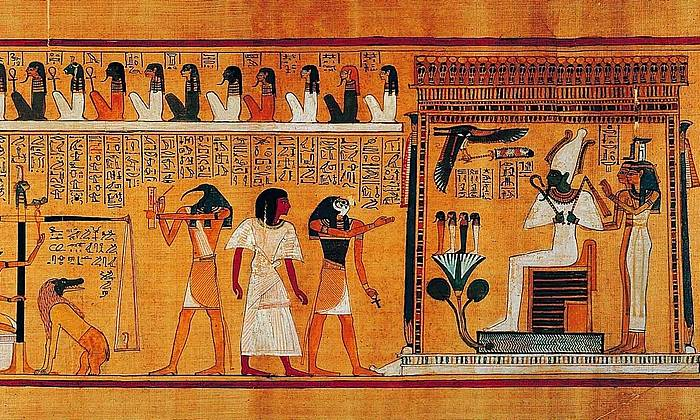
\includegraphics[width=0.8\linewidth]{egyiptom}
	\end{figure}
	
	
	\subsubsection{Az ókori görög festészet jellemzői}
	
	\begin{compactitem}
		\item Növény- és állatmotívumos díszítés a leggyakoribb.
		\item A megmaradt emlékek közül a legjelentősebb alkotások a festett vázák.
		\item A vázaképke a görög élet és mitológia érdekes jeleneteit mutatják be.
		\item Archaikus kor: feketealakos vázafestés (eredeti/fehér csempeszín + fekete vázafestés).
		\item Klasszikus kor: vörösalakos vázafestés (fekete háttér + vörösre festett alakok).
	\end{compactitem}


	\subsection{Az egyiptomi falkép elkészítésének munkamenete}
	
	Az egyiptomi vakolatok fő anyaga a nílusi iszap: agyag, homok, mész és gipsz keveréke. A kötőanyag kérdése eldöntetlen, lehet gipsz is, mész is.
	
	\begin{itemize}
		\item \textbf{A fal előkészítése:} 
		\begin{compactitem}
			\item Sima kőfelület esetén: vékony gipsz vakolat.
			\item Durva felület esetén: agyagos, vastagabb simító vakolat, erre vékony gipszes vakolás. Ilyen felületeken az esetleges domborítás a vakolatból készült.
		\end{compactitem}
		
		\item \textbf{Festék:} tempera.
		
		\item \textbf{Pigmentek:} okkerek, korom, mész, egyiptomi kék és zöld.
		
		\item \textbf{Előrajz:} fonalpattintással jelölték ki a főbb tengelyeket
		valamint a szinteket, és alakították ki a figurák arányait megadó hálózatot. A kompozíciót vörös festékkel rajzolták fel, és feketével korrigálták.
		
		\item \textbf{Festés:} először az alapszíneket festették fel síkszerűen és
		fedő módon. Az előrajzok ettől teljesen eltűntek. Ezután az egyre finomabb részletek, majd pedig a végső kontúrok következtek.
		
		\item \textbf{Lakkozás:} a sárga és vörös felületeken a 18. dinasztia idejében gyakran előfordul, a sárgák esetében talán az arany-
		hatás imitálására. A Nefertari sír sárga és vörös felületein gyantát és tojásfehérjét találtak a lakkozott felületeken, de korukat nem tudták megállapítani. Lehettek esetleg későbbi fixálások eredményei is.
	\end{itemize}
	
	\subsection{Színek az ókori egyiptomban}
	
	A színnek szinte minden kultúrában szimbolikus jelentése is van. Az alkimista irodalomban a vörös többnyire az aranyat, a fehér vagy a kék a higanyt vagy az ezüstöt jelöli. Az ókori Egyiptomban is gyakran mágikus-vallásos eszmék szabták meg a színek alkalmazását. A pigmentek nem a ritkaságuk miatt váltak értékessé, hanem a szín misztikus hatalma miatt, amely arra késztette az embert, hogy a pigmentek készítésekor legyõzze a nehézségeket.
	
	\subsubsection{Vörös és fehér}
	A predinasztikus idõkben Felsõ-Egyiptom fáraója "fehér" koronát viselt; a "vörös" korona az Alsó-Egyiptom fölötti uralmat szimbolizálta. Mindkét szín Hórusz szemét, az élet fenntartását jelképezte; a vörös a fehér komplementere volt.
	
	Amikor Menész egyesítette a két birodalmat (Kr. e. 2900 körül), kettõs koronát alkottak, amelyben a korábbi két korona úgy jelent meg, hogy egyik se domináljon a másik felett. A tisztaságot és spiritualitást jelképezõ fehér hatalmával egyesült a vért, tüzet és csillogást szimbolizáló vörös hatalma.
	
	Az egyiptomi mitológiában az oroszlán gyakran a szent helyek õreként jelenik meg. A Szfinx alakjában az oroszlán megtartotta az õr funkciót, de a Napisten jellemzõit is felvette. Úgy gondolták, hogy a fej Khafré fáraó idealizált portréja, a fáraót pedig a Napistennel azonosították. Ezért nem meglepõ, hogy a Szfinx arcán még most is feltûnnek a vörös festék nyomai. A vörös itt a felsõbb hatalmat, a védelmet, a tüzet, a parancsot jelképezi.
	
	A színek szimbolikája az orvoslásban is megjelent. Az õsi Egyiptomban gyakoriak voltak a vörös amulettek. A hit szerint ezek megóvták a katonákat a sebesüléstõl és elállították a vérzést.
	
	A vöröshöz kétféle konnotáció járult. Ha a Napot jelképezte, a szemhez kapcsolódott vagy amulettként használták, jót jelentett. Ha azonban Széth, Ozirisz gyilkosának színeként alkalmazták, gonoszságra utalt.
	
	Az ókori Egyiptomban a férfiak húsát általában vörössel jelenítették meg, a nõkét sárgásfehérrel. Néhány évezreddel késõbb, Kelet-Angolában is hasonló megkülönböztetést használtak: a fehér az élet, az egészség, a holdfény és a nõk színe volt, a vörös betegséghez, a Naphoz és a férfiakhoz kötõdött.
	
	Egyiptomban a legfontosabb vörös pigment a vízmentes vas(III)-oxid volt. A falfestményeken és a festett tárgyakon már a predinasztikus idõkben (Kr. e. 5000–3000) megjelent. Késõbb, a Kr. e. II. évezred táján  realgárt, arzén-szulfidot (As2S2) is használtak. Ez élénkebb színû volt a vas-oxidnál.
	
	A fehérhez két természetes pigmentet, krétát (kalcium-karbonátot) és gipszet (kalcium-szulfátot) használtak. Egyes feltevések szerint mesterségesen elõállított, fehér ólom-karbo- náttal is dolgoztak.
	
	A kis tárgyakat nem agyagból, hanem úgynevezett egyiptomi fajanszból készítették. A mázzal bevont tárgyakat sokféle anyaggal színezhették. A vörös és a barna máz alapja a vas-oxid volt. A két színt csak a VIII. dinasztiától (Kr. e. 1567–1320) tudták szándékosan megkülönböztetni: korábban a mester nem lehet biztos abban, hogy vörös vag barna lesz-e a kész edény. Az idõk folyamán kísérletezhették ki, hogy akkor válik élénk vörössé a máz, ha a vas-oxidhoz meghatározott arányban kálium-oxidot, mangán-monoxidot és ólom-oxidot adnak. A kálium-oxid a hamuzsír (kálium-karbonát) hõbontásakor keletkezett. A hamuzsír vagy az üveggyártáshoz használt egyiptomi homok szennyezése volt, vagy növényi hamu formájában használták fel. A mangán-monoxid az üveghez adott piroluzitból (mangán-dioxid), az ólom-oxid a galenitbõl (ólom-szulfid) képzõdött.
	
	A fehér fajansz gyártásakor többnyire nem adtak átlátszóságot csökkentõ anyagot a mázhoz, inkább finomra õrölt kvarcot használtak, amit vastag, üveges, átlátszó "héjjal" borítottak.
	
	\subsubsection{Fekete}
	
	A fekete fogalma elsõsorban a gonoszsághoz kötõdött. A sakálfejû istent, Anubiszt, a halál hercegét feketére színezték. De a vöröshöz hasonlóan a feketének is ambivalnes konnotációja volt. A betegek szívére gyakran tettek fekete skarabeuszt védelem gyanánt.
	
	Fekete pigmentként eleinte kormot használtak. Késõbb nagy mennyiségû piroluzitot adtak az üveghez, majd a vas(III)-oxid szabályozott redukcióját is rendszeresen alkalmazták. Az eljárás során nagy mennyiségû vas(III)-oxidot kellett magas hõmérsékleten redukálni, és az anyagnak addig kellett redukált állapotban maradnia, amíg a máz meg nem keményedett. Enyhe oxidáció mellett kék és zöld szín is keletkezhetett.
	
	\subsubsection{Sárga}
	
	Ez a szín a Napot, a boldogságot és a gazdagságot jelképezte.  A XVIII. dinasztia elõtti idõkben egyetlen sárga pigment volt csak, az okker (hidratált vas(III)-oxid). Késõbb felfedezték, hogy  az auripigment (arzén-triszulfid) és az ólom-antimonát sárgára színezi az üveget.
	
	\subsubsection{Kék}
	
	Az isteni igazságot jelképezõ kék az egyik legfontosabb szín volt. A sírokból számos kék tárgy került elõ. A kék amulettek viselõi az istenek oltalma alatt álltak.
	
	Az egyiptomiak tudták, hogy a lapis lazuli (lazúrkõ) az ultramarin festék alapja, de ritkasága miatt keves lapis lazulit használhattak. Ismerték az azurit (bázisos réz-karbonát) ásványt is, de tisztában voltak csekély kémiai ellenállásával és halvány színével is. A kék azonban annyira fontos volt, hogy kikísérletezték a híres egyipomi kék festéket.
	
	A vizsgálatok szerint ez a festék jól definiált kristályszerkezettel rendelkezõ kalcium-réz-tetraszilikát (CaCuSi4O10 vagy CuO, 4SiO4). A feljegyzések szerint elõször a IV. dinasztia idején (Kr. e. 2613–2494) alkalmazták.  Elõállításának titka azonban a Kr. u. IV. században elveszett, és csak a XIX. században fedezték fel újra. Az elemzések arra utalnak, hogy szilícium-dioxidot, réztartalmú malachitot vagy azuritot és kalcium-karbonátot hevítettek együtt. A nyersanyagoknak a lehetõ legjobban meg kellett közelíteniük az 1 CaO, 1 CuO, 4 SiO2  sztöchiometriai arányt, és kis mennyiségû folyósítószerre (sóra, boraxra) is szükség volt, hogy a kristályosodást szabályozzák. Az élénk kék szín elõállítása érdekében 1000 oC alatt, oxidáló atmoszférában kellett végezni az eljárást.
	
	A XVIII. dinasztia alatt már a kobalt volt a fajansz fõ színezõanyaga (kobalt-oxid formájában). Rendszerint bõségesen adtak hozzá rezet is. 0,05 százalék kobalt-oxid már élénk színt keltett, 0,2 százalék pedig lilára festette az anyagot. A kobalttal festett fajansztárgyak sötétkék színe a lapis lazulira emlékeztetett. A réz világosabbra, türkizesre változtatta a színt.
	
	\subsubsection{Zöld}
	
	Az egyipomiak a Nílus vidékét festették meg zölddel a freskókon. Ozirisz, a halál és a termékenység istenének színe ugyancsak a zöld volt. A zöldnek gyógyító erõt is tulajdonítottak. Az örök életet jelképezõ skarabeuszokat gyakran zöldre festették.
	
	A zöldet vagy porrá tört malachitból, vagy mesterséges zöld üvegzománc-õrleménybõl állították elõ. Néha az egyipomi kék és az okker keveréke adta ki a zöld színt. Máskor krizokollát (réz-szilikátot) is használtak, de ez az ásvány ritka volt Egyiptomban.
	
	Nofretete mellszobrának zöld fejdíszét elsõsorban bázisos rész-acetáttal (patinával) színezték. A festék valószínûleg úgy készült, hogy a rezet a bor seprõjében áztatták, majd a zöld felületi réteget lekaparták.
	
	A fajanszhoz réz-oxidot és vas(III)-oxidot is használtak zöld pigmentként. Késõbb a vas-oxid mennyisége jelentõsen megnõtt: valószínûleg rájöttek, hogy a vegyület erõsíti a zöld hatást. A sárga ólom-antimonát pigment felfedezése nyomán a zöld színárnyalatok skálája is gazdagodott.
	
	\subsection{The Painter in ancient Egypt} 
	

	Ancient Egyptian wall paintings provide a fascinating glimpse into the past. In tombs it was the painter's task to preserve the dead individual's spirit. Most tomb art generally followed consistent rules and held special meaning to the ancient Egyptians.
		
	\begin{wrapfigure}{r}{6cm}
		\centering
		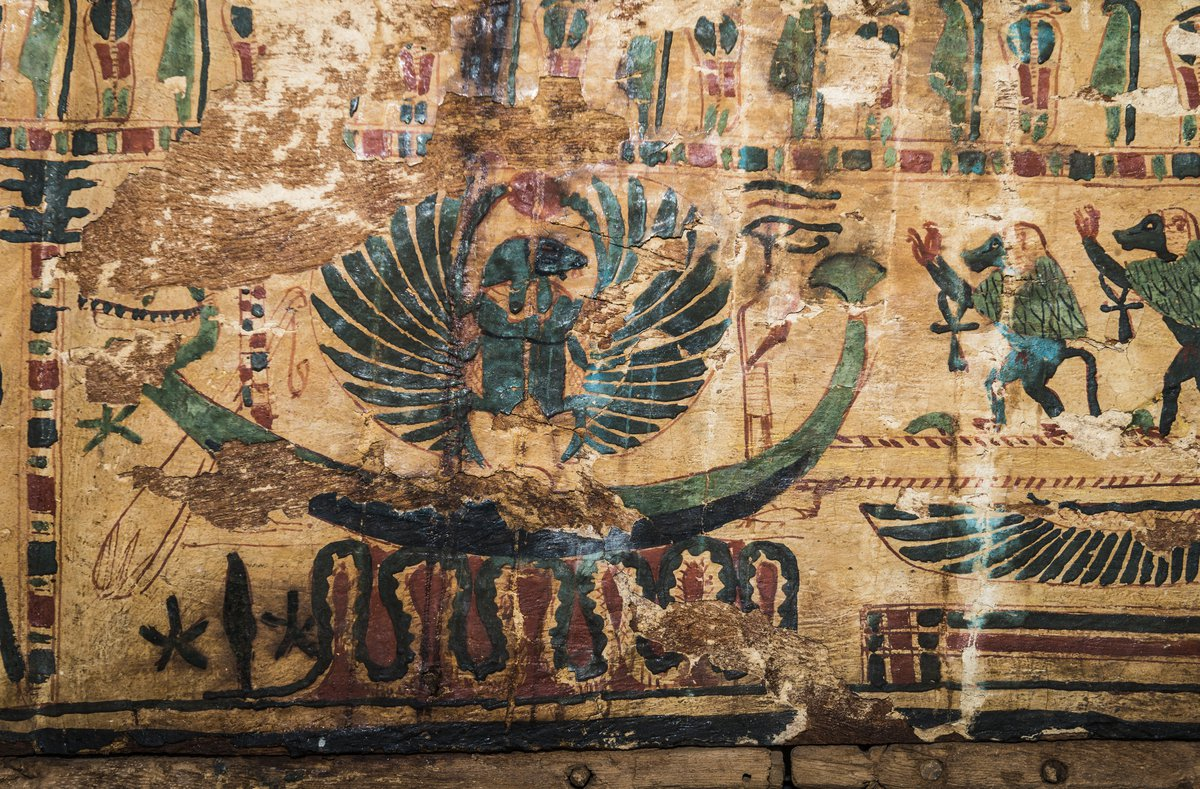
\includegraphics[width=1.0\linewidth]{egypt}
	\end{wrapfigure}
	The front and profile viewpoints depicted in a single human figure are one of the most characteristic features of Egyptian art. This is reminiscent of the fact that the ancient Egyptians saw the world in terms of dualities: life and death, flood and drought, good and bad. These composite images of the most recognisable parts of the human body were more detailed than a realistic pose and assisted the tomb owner’s ka (spirit) to recognise its body.

	\subsubsection{Size matters}
	
	Perspective and the status of figures were shown in a system of strips that looks much like a series of comics or a graphic novel. The use of perspective with a vanishing point was not used in Egyptian art. The lower border of a register was the ground line and depth was shown by the overlapping of figures or by figures stacked one above the other. The size of a figure indicated its relative importance in the image. Kings were portrayed larger than life to symbolise their god-like powers. Tomb owners, as the most important subject of the design, were also depicted on a grand scale. In contrast, wives and children, servants and animals were drawn smaller, indicating their lesser importance.
	
	\subsubsection{Grid system}
	
	Creating exact replicas of figures was critical. One way of ensuring correct proportion was to use a grid system – a set of vertical and horizontal lines painted onto the bare wall. This system allowed the initial draughtsman to faithfully copy and enlarge a design also overlaid with a grid. Cords soaked in red ink were stretched out between two pieces of wood and then snapped against the wall to create perfectly straight lines. These lines are sometimes still visible on unfinished walls.
	
	\subsubsection{A divine palette}
	
	The ancient Egyptians used colour not only for its aesthetic appeal but also for its perceived meaning. Both warm and cool colours were used, offering depth and interest to their art as well as signs to their gods. The Egyptians believed that certain colours were not merely symbolic of but were imbued with specific powers or attributes that were linked to various gods. As a result, great power could be contained within an object if it was made or painted in meaningful colours.
	
	The pigments used to make various colours consisted mainly of minerals that occur naturally in Egypt and surrounding areas. Minerals were ground up in a stone mortar and mixed in pots with water and an adhesive such as wood gum or egg white. Paint made in this way was called ‘tempera’.
	
	\subsubsection{Colours – their source and meaning}
	
	\begin{itemize}
		\item \textbf{White} was made from calcium carbonate (lime) or calcium sulphate (gypsum) and equalled purity. Calcite (also called Egyptian alabaster) was also used.
		
		\item \textbf{Yellow} was made from ochre while a bright, golden yellow was made from orpiment. Pale yellow was made from jarosite. Yellow was used to depict female flesh while golden yellow and gold itself was used to represent the sun and flesh of gods, particularly Re the sun god. Gold was considered a divine metal because it never tarnished.
		
		\item \textbf{Silver} was very rare in Egypt - it could be even more precious than gold. It was thought to be what the gods' bones were made from.
		
		\item \textbf{Blue} was made with azurite (copper carbonate) and represented the heavens, vegetation, youth, water and the Nile River. The colour known as Egyptian blue was made from heating quartz, ground malachite and calcium carbonate together. The finer the grain, the paler the blue.
		
		\item Blue was made with azurite (copper carbonate) and represented the heavens, vegetation, youth, water and the Nile River. The colour known as Egyptian blue was made from heating quartz, ground malachite and calcium carbonate together. The finer the grain, the paler the blue.
		
		\item \textbf{Green} was created with copper or by grinding up malachite and stood for Osiris, eternal life, prosperity and resurrection. It also represented regeneration and fertility so this colour was sacred to the goddess Hathor and was used to depict the flesh of Nephthys – the goddess of rebirth.
		
		\item\textbf{ Red} was made with ochre, just like yellow. Ochre gives a range of colours from yellow to red to dark brown, depending on the amount of water used. Iron oxide was also often used. During the New Kingdom, realgar was used for red but it fades to yellow over time. Red was used to paint male skin tones. It also represented the sun, evil, power, blood and life force.
		
		\item \textbf{Black} was made from soot or charcoal and signified Egypt’s ancient name ‘Kemet’ or ‘black land’ and the silt-fed soil around the Nile. Black was also used to denote the underworld and Osiris.
	\end{itemize}

	\subsubsection{Forrás}
	
	\href{https://australian.museum/learn/cultures/international-collection/ancient-egyptian/the-painter-in-ancient-egypt/}{Australian museum}
\newpage

\section{Pompejiben feltárt falfestmények négy meghatározó festészeti stílusa }

	\subsection{A tétel teljes címe}
	
	Beszéljen a Pompeiiben feltárt falfestmények alapján a négy meghatározó festészeti stílusáról!
	
	\subsection{Bevezetés}
	
	A falfestés stílusai Pompejiben - a római festészet legszebb emlékeit Pompejiben és
	Herculaneumban láthatjuk - a Vezúv Kr. u. 79-ben betemette a városokat, majd 1748-ban
	fedezték fel - a falfestmények négy különböző stílust képviselnek, külön és keveredve is
	előfordulnak.
	
	\subsection{Összefoglalás}
	
	\begin{enumerate}
		\item  \textbf{Inkrusztációs stílus} - a falfestmények berakásokat utánoznak, márványból készült
		falburkolat hatását keltik.
		
		\item  \textbf{Architektonikus stílus} - építészeti elemek ábrázolásával látszólag bővítették a teret. 
		
		\item \textbf{ Ornamentális stílus} - mitológia jeleneteket feldolgozó dekoratív stílus, keretezet
		táblakép illúzióját keltve.
		
		\item\textbf{ Illuzionisztikus stílus} - tájképek, csendéletek, épületek valószerűen ábrázolt látszatát
		festették - a mélység irányába futó vonalak párhuzamosak (axonometria) - használták a
		színperspektívát.
	\end{enumerate} 

\begin{figure}[H]
	\centering
	\includegraphics[width=1.0\linewidth]{"Pompeji 4 stilusa"}
\end{figure}


	\subsection{A falfestészet}
	
	A pompeji ház minden szobáját kifestették, kivéve a gazdasági rendeltetésű helyiségeket
	(éléskamra, konyha), valamint a rabszolgák lakószobáit. A falfestészet korántsem volt
	állandó jellegű a város egész fennállásának folyamán: változott a megrendelők társadalmi
	helyzete, változott az ízlés és ezzel együtt a festészet stílusa is változásokon ment
	keresztül. A festők általában a freskó-technikát alkalmazták: a friss vakolatra festettek.
	Az alapot előzőleg különleges eljárásokkal megdolgozták, hogy egy ideig friss maradjon,
	s ne kezdjen száradni már a képfestés közben. A pompeji falfestmények frissen csillogó
	színei részben az alap előzetes preparálásának tulajdoníthatók, részben azonban annak is,
	hogy a festékek kitűnő minőségűek; a jó festékkeverés nemzedékek kitartó
	fáradozásainak és kísérletezéseinek volt az eredménye.
	
	
	Pompejiben több szépmíves műhely vagy „iskola” működött, melyek mindegyike
	kialakította a maga külön művészi szabályait s tagjaik szigorúan ragaszkodtak ezekhez. A
	művészi önállóság csupán abban nyilvánulhatott meg, hogy a művész a saját
	egyéniségének megfelelően kombinálta és fejlesztette a hagyományos motívumokat. 
	Pompeji persze nem volt hangadó centrum; a Rómában uralkodó áramlatokat követte,
	Róma pedig a Görögországból és a hellénisztikus Keletről származó irányzatokat. A
	pompeji falfestészetben négy stílust különböztetünk meg.
	
	\subsection{Inkrusztációs stílus}
	
	Az első stílus az „inkrusztációs stílus” nevet kapta. Lényege abban áll, hogy a falak
	vakolatát márványszerűen festették ki, s ily módon a falak azt a benyomást keltik a
	szemlélőben, mintha márványlapokból lennének összeillesztve. A falfelületet először
	több mezőre osztották, melyeket különféle módokon lehetett kialakítani; majd az egyes
	mezőket tarka színekkel bemázolták, s márvány-ereket utánzó vonalakkal hálózták be.
	Ennek a stílusnak jó példáját láthatjuk Sallustius házának tablinumában.
	
	
	A faltő végig sárga, fölötte fekete márványtáblákat utánzó széles sáv húzódik, majd több
	sorban elhelyezett keskeny, különböző színű (sárga, zöld, lila) téglalapok következtek. A
	festőn kívül még stukkókészítő mester is közreműködött a ház díszítésében. A fal felső
	részén stukkóból formált párkányfogazat vonul végig, fölötte ismét színes „márványtáblák” sorai helyezkednek el, majd újra párkányzat következik. Ily módon a
	falnak mintegy kétharmadát díszítések borítják.
	Ennek a stílusnak teljes-kibontakozását főleg Délos szigetén és a kisázsiai Priéné
	városban épült hellénisztikus házak falain figyelhetjük meg. Itáliai változata - melyet
	éppen Pompejiben ismerhetünk meg legjobban - kiváltképpen a tisztán architektonikus
	részleteket kedvelte: a fal függőleges voltát kihangsúlyozó oszlopokat és pilléreket.
	Ezeket elsősorban ajtók, ablakok, fülkék keretezésére alkalmazták, valamint a fal felső
	részén, az első és a második párkányzat között. Általában véve ez a stílus kissé merev.
	Súlyossága idővel fárasztónak hat, s a fal unalmasnak tűnik.
	
	\subsection{Architektonikus stílus}
	
	A második stílus (i. e. II. század vége) elhagyta a stukkó-párkányzatokat, és az első
	stílusnak csupán a festészeti elemeit alkalmazta Tisztára architektonikus festészetnek
	lehet nevezni. Az első stílus „megszilárdította” a falat, korláttá varázsolta, mely a
	helyiséget elválasztotta a külvilágtól; a második stílus azonban eltávolította ezt a korlátot.
	Az oszlopok, féloszlopok és pillérek most már nem csupán az ajtókat keretezték be, s
	nemcsak a fal felső részének díszítésére szolgáltak; a művész az egész falfelületet
	befestette velük a faltőtől - sőt néha a padlótól - egészen a mennyezetig.
	Az arányok gondos mérlegelése és az árnyékok művészi elosztása folytán az igazi fal
	eltűnt, s mint a színpadi dekorációknál, elrejtőzött a művész alkotta látszatvalóság
	mögött. A festő a perspektíva eszközeivel a térbeli mélység illúzióját varázsolja a néző
	szeme elé. A második stílus további fejlődése folyamán a falon monumentális épületek
	jelennek meg térbeli egymásmögöttiségben elrendezve: a szemlélőben elenyészik a fal
	határoló, korlátozó jellegének érzete. A fal közepére - az épületek közé - rendszerint zárt
	ajtót festett a művész. A második stílus utolsó periódusában ez az ajtó „megnyílt”, s a
	szemlélő rajta „kitekintve” fákat, embereket, állatokat - tájakat és mitológiai jeleneteket
	láthatott.
	
	
	A második stílus két különböző elemet egyesített: az architektonikus perspektívát és a
	monumentális falfestészetet, melynek az előbbi keretül szolgált. E stílus sikerének titka
	részint a faldekorációk gondolati egyszerűségében és tisztaságában rejlik, részint pedig
	abban, hogy a művészek pompás architektonikus képeiknek meg tudták adni azt a 
	perspektivikus mélységet, mely gyakran csalódásig híven utánozza a valóságot. Ezek az
	architektúrák nemcsak a falakat „szüntették meg”, hanem magát a helyiséget is - olyan
	kilátóponttá varázsolták, ahonnan gyönyörködni lehetett büszke paloták szépségében és a
	mögöttük elterülő táj végtelenbe nyúló messzeségében. Ennek a stílusnak Kis-ázsia
	hellénisztikus központjaiban volt a hazája; bajosan lehetett volna még egy ilyen festészeti
	stílust találni, amely ennyire illett volna a római uralom terjeszkedési korához.
	
	\subsection{Ornamentális stílus}
	
	A harmadik stílus bizonyos értelemben tiltakozást fejezett ki a második ellen. Az utóbbi
	stílus - mint mondottuk - „eltűnteti” a falakat: a térbeli mélység illúzióját keltő
	épületekkel festi tele őket, melyek mögött még tájak és emberek láthatók. Ezzel szemben
	a harmadik stílus sohasem téveszti szem elől, hogy a fal mindenek előtt sík felület: tehát
	nem „töri át” sehol, s nem törekszik térbeli, perspektivikus hatásokra. A harmadik stílus
	tökéletes példáját láthatjuk a „Százéves jubileum házában”, ahol a fő mező fekete
	hátterén mintegy elenyészve apró fehér figurák állnak. Ennek a stílusnak a dekorációi
	faliszőnyeget utánoznak.
	Pompejibe természetesen voltak igazi faliszőnyegek is, de egy sem maradt meg; csak a
	falba vert szögek és a kampók jelzik egykori helyüket. A művész egész képsorozatokat
	ábrázolt faliszőnyeg-utánzatán. De hiába keresnénk köztük a római történelemből vagy a
	helyi krónikából vett jeleneteket viszont majdnem az egész görög mitológiát láthatjuk
	rajtuk, főleg szerelmi történeteket, melyek Ovidius mitológiai költészetének szellemét
	sugározzák. 
	
	\subsection{ Illuzionisztikus stílus}
	
	A negyedik stílus korai formájának kell tekintenünk azt a kísérletet, amely a „szőnyegelv” és a perspektíva összeegyeztetésére törekedett. Ez persze megvalósíthatatlan, mert a
	perspektíva „kitárja”, a „szőnyeg” ellenben „bezárja” a falat. Ennek a próbálkozásnak
	egyik példáját láthatjuk Lucretius Fronto házában. A faltő helyett csupán keskeny sáv fut
	végig a padlózat fölött; a fal öt mezőre van tagolva; a középső mező sötétpiros „szőnyeg”, rajta Dionysost és Ariadnét ábrázoló kép; ettől jobbra és balra egy-egy fekete „szőnyeg”, arany kandeláberekkel és kis tájképekkel díszítve.
	A negyedik és az ötödik sávban architektonikus motívumok szerepelnek: alul nagy ablak
	oromtetővel; fölötte - a perspektivikus ábrázolás halvány visszfényeként - egy kerek
	épület ión oszlopai, melyek túlságosan vékonyak ahhoz, hogy valóságérzetet
	kelthessenek; a körbefutó virágfüzérek még csak jobban kihangsúlyozzák az
	architektonikus motívum valószerűtlenségét. Éppen ilyen fantasztikusak a felső fríz
	épületei, bár közöttük valóságosan létező típusokat is lehet látni: a középen egy
	háromajtós bazilikát, s mindegyik oldalon egy-egy ctediculát, felettük fedélszerkezettel.
	Ám a bazilika közepét kis csendélet foglalja el, fölötte pedig háromlábú üst (tripus)
	látható - mintha a művész figyelmeztetni akarná a nézőt, hogy kompozícióját
	semmiképpen ne tekintse egy valóságos épület ábrázolásának.
	
	A harmadik stílus - melynek finomságát Pompejiben meg sem közelíti a többi - túlságosan „akadémikus” volt ahhoz, hogy nagy sikerre számíthatott volna. S ha a
	köztársaság korának megrázkódtatásaitól, a császárság korának üldöztetéseitől kimerült 
	régi arisztokrácia a házaiba vonult vissza, hogy legalább otthon élvezzen ideig-óráig
	nyugalmat, biztonságot és békességet - az Imperium támogatását élvező kereskedelem és
	ipar képviselői még otthonukban sem óhajtottak elszakadni a világtól; házi kényelmet
	akartak, de nem kívántak lemondani a világ csábító messzeségeiről.
	A „szőnyeg-stílus” és a perspektíva összehangolására irányuló kísérlet ebből a
	szemléletből, ebből a lelki beállítottságból fakadt. A város pusztulása természetesen véget
	vetett a pompeji falfestészet további fejlődésének. Itt-ott meg lehet figyelni újabb stílusok
	csíráit, de ezek már nem bontakozhattak ki.

\section{Források}

\textit{(Nem teljes.)}

\begin{itemize}
	\item \href{https://www.kinvaart.hu/1-lecke-muveszettortenet-ingyenes-online-festeszeti-tanfolyam/}{Kinva art}
	\item \href{https://www.kfki.hu/~cheminfo/hun/teazo/uj/szin.html}{Színek az ókori egyiptomban}
	
	\item 
	\href{http://aktivitas-tiszk.hu/elearning/Bergendi_Rita/Okor.pdf}{Művészettörténet a kezdetektől az ókor végéig}
	
	\item 
	\href{http://mek.oszk.hu/14000/14064/14064.pdf}{Kovács Nemere: A képzőművészet története}
	
	\item
	\href{https://australian.museum/learn/cultures/international-collection/ancient-egyptian/the-painter-in-ancient-egypt/}{Australian museum}
\end{itemize}


\end{document}
